
%EACH CHAPTER CAN HAVE SECTIONS. EACH SECTION CAN HAVE MORE THAN ONE SUBSECTION AND EACH CHAPTER CAN HAVE MORE THAN ONE SECTION
%EXAMPLE
% \chapter{Introduction}
% \section{Need}
% \subsection{Social Engineering}


\chapter{Introduction}

\section{Need}

\subsection{Social Engineering}
Social Engineering is the act of manipulating a person to take an action that may or may not be in the targets best interest. This may include obtaining information, gaining access, or getting the target to take certain action\cite{book_se}

\subsection{Current Scneario}
Businesses spend a significant portion of their annual information technology budgets on high-tech computer security. But the firewalls, vaults, bunkers, locks and biometrics those dollars buy can be pierced by attackers targeting untrained, uninformed or unmonitored users. Humans are the weakest link in any security system, according to KL-based organizers of the Hackers Halted Asia Pacific 2009 conference.\cite{link_humanweak}\\[0.5cm]
The chief minister of Malacca, Datuk Seri Haji Mohd Ali Bin Mohd Rustam, said there is no perfect system in the world. ”Even if you have the best security devices and software–your organization still relies on humans–who are the weakest link in any security system. Public education and awareness is essential.”\\[0.5cm]
Figure \ref{fig:data} is a Data Security Breach Statistics of 2008 revealing that Malicious Insider and Careless/Untrained Insider is a bigger threat than an outside cracker.\\[0.5cm]
Also, in the age of Social Networking Sites like Facebook, Twitter, Linkedin, Google+ information of companies internal hierarchy structure, employees,
\begin{figure}[htb]
\centering
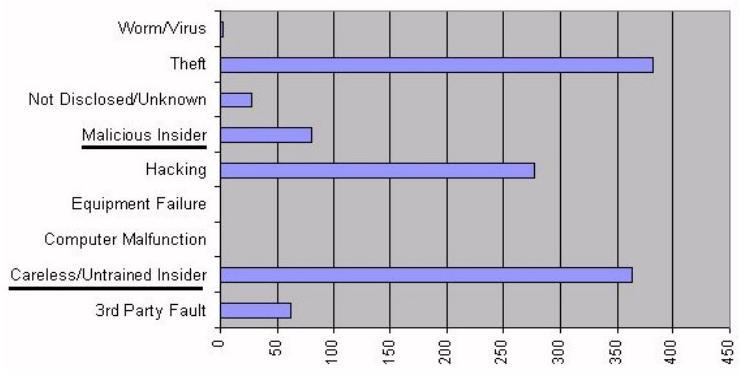
\includegraphics[scale=0.6]{project/diagrams/figdata}
\caption{Figure 1.1: Data Security Breach Statistics of 2008}
\label{fig:data} %see below of how to use it
\end{figure}
personal information is readily available online for the information gathering phase to breach companies security perimeter by various social engineering ways like phishing links, Trojans, Backdoors, Password guessing, breaking security questions etc.\\[0.5cm]
Is it possible to break into the circle of friends network on social networking sites and make them reveal certain information about them which can be used further to infiltrate the security perimeter of a company?\\[0.5cm]
Our project is designed to answer this Question and provide a Proof of Concept that Yes, it can be done and without even raising any suspicion on the target for a long time.


%\ref is used to refer to the \label of an image, below is an example
%Figure \ref{fig:data} is a Data Security Breach Statistics of 2008 revealing that Malicious Insider and Careless/Untrained Insider is a bigger threat than an outside cracker.
%BLAH BLAH

\section{Basic Concept}
In this project we will use two main concepts:

%BLAH BLAH
\subsection{Profile Hijacking}
%BLAH BLAH

In Profile Hijacking, we will impersonate the target(s) profile on Social Networking Sites like Facebook and use their identity to infiltrate the network of other targets friend to fit in the group. Profile Hijacking is important, to use them to reveal certain information without their knowledge.\cite{paper_allyourcontacts}


\subsection{Using Humans as Botnets}
%BLAH BLAH

We studied many AI based Chat Bots that are available on the web and we found that Using Chat Bots to chat with humans for Social Engineering Attack is not feasible as Humans detect that the other person is not a human but a program and hence the attack fails even before it is launched.\cite{paper_towardsautomating}\\[0.5cm]
Since developing a fully convincing AI based Chat Bot is not possible considering the Scope, we will use another human to do the talking with our target while we sit in between, watch and modify the conversation towards the conversation which would reveal certain information which we are interested in.\cite{paper_honeybot}


\section{Application}
%BLAH BLAH
Some of the best tools for fighting social engineering attacks are security awareness training and social engineering testing. The effectiveness of these controls will vary based on the quality of their implementation, including follow-up and retraining.\\[0.5cm]
Social engineering testing, by its very nature, can be difficult to conduct without third-party assistance. One option is to engage an information security organization to conduct testing. The testing can uncover areas in which an organization is most vulnerable so that risk can be assessed and mitigation strategies can be formulated and implemented.\\[0.5cm]
Rolling social engineering testing into a larger security penetration engagement can reduce the cost of the social engineering component, says Jim Patterson, director of consulting for Rapid7.\cite{link_humanweak}\\[0.5cm]
Main Application of this Project is to develop a tool that will aid in doing Social Engineering Testing on Companies Employees, also it will provide as a live demonstration to employees under training on how social engineering can be done and how by being cautious one can prevent serious damage not only to the company but also to their private life.\\[0.5cm]